\documentclass{article}
\usepackage{graphicx} % Required for inserting images

\title{classy}
\author{acondolu}
\date{March 2024}

% Imports
\usepackage{amssymb}
\usepackage{amsthm}
\usepackage{amsmath}
\usepackage{mathtools}
\usepackage{bussproofs}
\usepackage{tikz}
\usetikzlibrary{fit}

% General math notation
\newtheorem{definition}{Definition}
\newtheorem{example}{Example}
\newtheorem{theorem}{Theorem}
\newcommand\defeq\coloneqq
\newcommand\treplace[1]{\left\{#1\right\}}
\newcommand\lat{$\lambda$-term}
\newcommand\lats{$\lambda$-terms}
\newcommand\clat{classy-term}
\newcommand\clats{classy-terms}
\newcommand\clapp{classy-program}
\newcommand\claps{classy-programs}


% Classy specific notation

\newcommand{\mytt}[1]{\mbox{\texttt{#1}}}
\newcommand{\ca}[2]{\mytt{<} #1, #2\mytt{>}}
\newcommand{\cs}[2]{\mytt{[}#1, #2\mytt{]}}
\newcommand{\ee}[0]{\blacksquare}
\newcommand{\contr}[1]{\mytt{\{}#1\mytt{\}}}
\newcommand{\wf}[0]{\mbox{ wf}}
\newcommand{\Cut}[0]{\parallel}
\newcommand{\Scope}[2]{#1\left(#2\right)}
\newcommand{\Result}[0]{\mathbb{R}}
\newcommand{\ltrans}[1]{\tau\left(#1\right)}
\newcommand{\ltransaux}[1]{\tau_{\mbox{aux}}\left(#1\right)}
\newcommand{\cuts}[0]{\Pi}


\begin{document}

\maketitle

\section{Calculus}

\begin{definition}[Terms]
\[ t, u ::= \ee \mid x \mid \ca t u \mid \cs t u \mid \contr {t, u}\]
\end{definition}

\begin{definition}[Types]
\[ A, B ::= p \mid \bar p \mid A \wedge B \mid A \vee B \]
\end{definition}

\begin{definition}[Dual type $A^\bot$].

\bgroup
\def\arraystretch{1.3}
\begin{tabular}{l c l}
   $p^\bot$ & $\defeq$ & $\bar p$ \\
   ${\bar p}^\bot$ & $\defeq$ & $p$ \\
   $(A \vee B)^\bot$ & $\defeq$ & $A^\bot \wedge B^\bot$ \\
   $(A \wedge B)^\bot$ & $\defeq$ & $A^\bot \vee B^\bot$ \\
\end{tabular}\egroup
    
\end{definition}

\begin{definition}[Typing rules].

\begin{prooftree}
\AxiomC{}
\UnaryInfC{$ x \colon A, x \colon A^\bot$}
\end{prooftree}

\begin{prooftree}
\AxiomC{$ \Gamma$}
\RightLabel{weakening}
\UnaryInfC{$\Gamma, \ee \colon A$}
\end{prooftree}

\begin{prooftree}
% \def\fCenter{\mbox{\ $\Rightarrow$\ }}
\def\fCenter{}
\AxiomC{$ \Gamma, t \colon A, u \colon A$}
\RightLabel{contraction}
\UnaryInfC{$\Gamma, \contr{t, u} \colon A$}
\end{prooftree}

\begin{prooftree}
\AxiomC{$ \Gamma, t \colon A, u \colon B$}
% \RightLabel{}
\UnaryInfC{$\Gamma, \cs t u \colon A \vee B$}
\end{prooftree}

\begin{prooftree}
% \def\fCenter{\mbox{\ $\Rightarrow$\ }}
\def\fCenter{}
\AxiomC{$ \Gamma, t \colon A$}
\AxiomC{$ \Delta, u \colon B$}
\RightLabel{}
\BinaryInf$\fCenter \Gamma, \Delta, \ca t u \colon A \wedge B$
\end{prooftree}

% \begin{prooftree}
% \AxiomC{$ \Gamma, t \colon \neg A$}
% \AxiomC{$ \Delta, u \colon \neg B$}
% \RightLabel{}
% \BinaryInf$\fCenter \Gamma, \Delta, \ca t u \colon \neg (A \vee B)$
% \end{prooftree}

% \begin{prooftree}
% \AxiomC{$ \Gamma, t \colon \neg A, u \colon \neg B$}
% % \RightLabel{}
% \UnaryInfC{$\Gamma, \cs t u \colon \neg ( A \wedge B)$}
% \end{prooftree}

\begin{prooftree}
\AxiomC{$ \Gamma, t \colon A$}
\AxiomC{$ \Delta, u \colon A^\bot$}
\RightLabel{cut}
\BinaryInfC{$\Gamma, \Delta$}
\end{prooftree}

\end{definition}

\newpage

% TODO: define cut expression

\begin{definition}[Programs]
    A \emph{cut expression} has the form $t * u$ where
    $t$ and $u$ are terms. The cut operator $*$ is commutative.

    Programs are denoted by $\Pi$ and are unordered
    sequences of cut expressions.
    \[ \Pi ::= \epsilon \mid \Pi, t * u \]
\end{definition}


\vspace{1em}
\begin{definition}[Reduction rules].\\[1em]
\bgroup
\def\arraystretch{1.3}
\begin{tabular}{l l c l l}
   Destruct & $\Pi,\ca {t_1} {t_2} * \cs {u_1} {u_2}$ & $\to_d$ & $\Pi, t_1*u_1, t_2*u_2$ \\
   Send & $\Pi, x * t$ & $\to_s$ & $\Pi\treplace{x \Leftarrow t}$ \\
   Copy & $\Pi,\contr{t_1, t_2} * u$ & $\to_c$ & $\Pi, t_1*u, t_2*u^\alpha$ \\
%    & $\Pi,\ca {t_1} {t_2} * \ee$ & $\to$ & $\Pi, t_1*\ee, t_2*\ee$ \\
%    & $\Pi,\cs {t_1} {t_2} * \ee$ & $\to$ & $\Pi, t_1*\ee, t_2*\ee$ \\
\end{tabular}\egroup\\

\noindent The Copy rule makes a copy of the term $u$ by
duplicating the free variables that occur in it.
We denote by $u^\alpha$ the term obtained from $u$ by replacing
each variable $x$ with a new fresh variable $x'$.
Note: if $u$ contains free variables, the notion of copy is
undefined at the moment (TODO).

\end{definition}

\begin{example}[Divergent program]

\[\omega \defeq \cs{\contr{\ca{x}{y}, x}}{y}\]

\bgroup
\def\arraystretch{1.3}
\begin{tabular}{rl}
    $\Omega \defeq $ & $\omega * \ca{\omega'}{\Result}$ \\
    $\to_d$ & $\contr{\ca{x}{y}, x} * \omega', y * \Result$ \\
    $=$ & $\contr{\ca{x}{y}, x} * \cs{\contr{\ca{x'}{y'}, x'}}{y'}, y * \Result$ \\
    $\to_c$ & $\ca{x}{y} * \cs{\contr{\ca{x'}{y'}, x'}}{y'}, x * \omega'', y * \Result$ \\
    $\to_d$ & $x * \contr{\ca{x'}{y'}, x'}, {y}*{y'}, x * \omega'', y * \Result$ \\
    $\to_s$ & $x * \contr{\ca{x'}{y'}, x'}, x * \omega'', y' * \Result$ \\
    $\to_s$ & $\contr{\ca{x'}{y'}, x'} * \omega'', y' * \Result$ \\
\end{tabular}
\egroup
\end{example}

\begin{definition}[$\alpha$-equivalence]
    We define $\equiv_\alpha$, the equivalence relation over \clats{} or \claps{} up to renaming of variables. (TODO)
\end{definition}

\section{Confluence}
Critical pairs may arise because of terms like:
\begin{itemize}
    \item $x * y$: not actually critical pairs, they are $\alpha$-equivalent.
    \item $\contr{t_1, t_2} * x$: invalid at the moment, because $x$ has a free variable (TODO).
    \item $\contr{t_1, t_2} * \contr{u_1, u_2}$: locally confluent.
\end{itemize}

\vspace{2em}

% Fun facts:
% \begin{itemize}
%     \item all variables are linear!
%     \item $Left(x) \equiv \cs{x}{\ee}$
%     \item $Right(x) \equiv \cs{\ee}{x}$
%     \item $Pair(a, b) \equiv \ca a b$
% \end{itemize}

\section{Embedding $\lambda$-terms}

An embedding of \lats{} into \claps{} can be defined through the
usual type embedding that translates $A \to B$ into $A \vee B^\bot$.

We denote by $\sigma$ a sequence of assignment of variables to terms
of the form $(x \mapsto t)$.

We denote by $\sigma_x$ the restriction of an assignment $\sigma$
to the variable $x$:
\[\sigma_x := \contr{t \mid (x \mapsto t) \in \sigma}.\]

The translation $\ltrans{t}$ of a $\lambda$-term into a program relies on an auxiliary function $\ltransaux{t}$, which takes
in input a $\lambda$-term and returns a thriple $(\cuts; \sigma; t')$ composed of a program, a substitution, and a term.

The auxiliary function $\ltransaux{t}$ is defined as follows:

\begin{center}
\bgroup
\def\arraystretch{1.3}
\begin{tabular}{lcl}
    $\ltransaux{\lambda x. t} $ & $\defeq$ & $(\cuts; \sigma \setminus \sigma_x; \cs{\contr{\sigma_x}}{t'}) $ \\
    & & where $(\cuts; \sigma; t') \defeq \ltransaux{t}$ \\
    $\ltransaux{x t_1 \ldots t_n}$ & $\defeq$ & $(\cuts_1\ldots\cuts_n; \sigma_1\ldots \sigma_n(x\mapsto\ca{t_1'}{\ldots\ca{t_n'}{z}}); z) $ \\
    & & where $(\cuts_i; \sigma_i; t_i') \defeq \ltransaux{t_i}$ for $i=1\ldots n$\\
    & & and $z$ is a fresh variable \\
    $\ltransaux{t_0 t_1 \ldots t_n}$ & $\defeq$ & $(\cuts_0\cuts_1\ldots\cuts_n, t_0' * \ca{t_1'}{\ldots\ca{t_n'}{z}}; \sigma_0\ldots \sigma_n; z)$ \\
    & & where $(\cuts_i; \sigma_i; t_i') \defeq \ltransaux{t_i}$ for $i=0\ldots n$ \\
    & & and $z$ is a fresh variable \\
    & & and $t_0$ is a lambda abstraction. \\
\end{tabular}
\egroup
\end{center}

The translation $\ltrans{t}$ is then defined as follows:

\[\ltrans{t} \defeq \cuts \mbox{ where } (\cuts; \sigma; t') \defeq \ltransaux{t}. \]

\section{Correctness}

\begin{definition}[$\Pi$-path]
    Let $\Pi$ be a program. A $\Pi$-path is given by:
    \begin{itemize}
        \item $n > 0$
        \item a sequence of variables $x_0, \ldots, x_n$ in $\Pi$
        \item terms $t_0 \circledast u_0, \ldots, t_n \circledast u_n$ in $\Pi$ (where $t \circledast u$ is either $\ca t u$ or $t * u$)
        \item such that $x_i \in t_i$ and $x_{i+1}\in u_i$ for $i=0\ldots n-1$.
    \end{itemize}
\end{definition}

\begin{definition}
    A program $\Pi$ is valid if
    \begin{itemize}
        \item All subterms are unique, except variables: each variable occurs exactly twice.
        \item There are no cyclic $\Pi$-paths (cyclic meaning a $\Pi$-path $x_0, \ldots, x_n$ such that $x_0 = x_n$).
    \end{itemize}
\end{definition}

\section{Simulation}

\begin{theorem}
    For every $\lambda$-terms $t$ and $u$, if $t \to_\beta u$,
    then $\ltrans{t} \to \ltrans{u}$.
\end{theorem}
\begin{proof}
    Let $C$ be an evaluation context such that $t = C\langle(\lambda x. t')u'\rangle$ and $u = C\langle t'\treplace{x\Leftarrow u'}\rangle$.
\end{proof}


\newpage

\section{Stub correctness proofs}

\begin{prooftree}
\AxiomC{}
\UnaryInfC{$ \Cut x, x $ \wf}
\end{prooftree}

\begin{prooftree}
\AxiomC{$\Pi \Cut \Gamma $ \wf}
\UnaryInfC{$\Pi \Cut \Gamma, \ee$ \wf}
\end{prooftree}

\begin{prooftree}
\def\fCenter{}
\AxiomC{$\Pi \Cut \Gamma, t , u $ \wf}
\UnaryInfC{$\Pi \Cut \Gamma, \contr{t, u}$ \wf}
\end{prooftree}

\begin{prooftree}
\AxiomC{$\Pi \Cut \Gamma, t , u $ \wf}
% \RightLabel{}
\UnaryInfC{$\Pi \Cut \Gamma, \cs t u $ \wf}
\end{prooftree}

\begin{prooftree}
\def\fCenter{}
\AxiomC{$ \Pi \Cut \Gamma, t $ \wf}
\AxiomC{$ \Pi' \Cut \Delta, u $ \wf}
\RightLabel{}
\BinaryInfC{$\Pi, \Pi' \Cut \Gamma, \Delta, \ca t u $ \wf}
\end{prooftree}

\begin{prooftree}
\AxiomC{$ \Pi \Cut \Gamma, t $ \wf}
\AxiomC{$ \Pi' \Cut \Delta, u $ \wf}
\BinaryInfC{$\Pi, \Pi', t * u \Cut \Gamma, \Delta$ \wf}
\end{prooftree}

\vspace{2em}

\begin{itemize}
    \item $x*a$
    \item $x*b$
    \item $<a, b>$
\end{itemize}

% \tikzset{> = stealth}
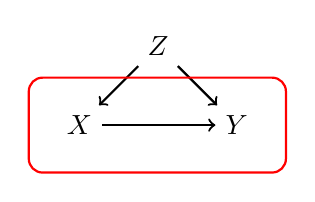
\begin{tikzpicture}[thick, box/.style = {draw,red,inner sep=10pt,rounded corners=5pt}]
    \node (x) at (0,0) {$X$};
    \node (y) at (2,0) {$Y$};
    \node (z) at (1,1) {$Z$};
    \path[->] (x) edge (y);
    \path[->] (z) edge (x);
    \path[->] (z) edge (y);
    \node[box, fit=(x)(y)] {};
\end{tikzpicture}

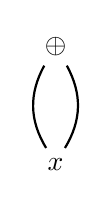
\begin{tikzpicture}[thick, box/.style = {draw,red,inner sep=10pt,rounded corners=5pt}]
    \node (z) at (0,1.5) {$\oplus$};
    \node (x) at (0,0) {$x$};
    \draw[-] (z) to [bend right=30](x);
    \draw[-] (z) to [bend left=30](x);
    % \node[box, fit=(x)(y)] {};
\end{tikzpicture}

\[T := \cs{\contr{\ca{-x}{-y}, +x}}{+y}\]

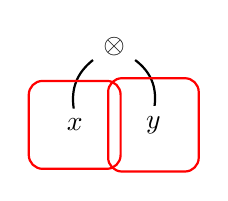
\begin{tikzpicture}[
    thick, box/.style = {draw,red,inner sep=10pt,rounded corners=5pt}
  ]
    \node (x) at (0,0) {$x$};
    \node (y) at (1,0) {$y$};
    \node (1) at (0.5, 1) {$\otimes$};
    \draw[-] (1) to [bend right=30](x);
    \draw[-] (1) to [bend left=30](y);
    \node[box, fit=(x)] {};
    \node[box, fit=(y)] {};
\end{tikzpicture}

\newpage

\begin{prooftree}
\AxiomC{}
\UnaryInfC{$ \Cut x, x $ \wf}
\end{prooftree}

\begin{prooftree}
\AxiomC{$\Pi \Cut \Gamma $ \wf}
\UnaryInfC{$\Pi \Cut \Gamma, \ee$ \wf}
\end{prooftree}

\begin{prooftree}
\def\fCenter{}
\AxiomC{$\Pi \Cut \Gamma, t , u $ \wf}
\UnaryInfC{$\Pi, \alpha=\contr{t, u} \Cut \Gamma, \alpha $ \wf}
\end{prooftree}

\begin{prooftree}
\AxiomC{$\Pi \Cut \Gamma, t , u $ \wf}
% \RightLabel{}
\UnaryInfC{$\Pi, \alpha=\cs{t}{u} \Cut \Gamma, \alpha $ \wf}
\end{prooftree}

\begin{prooftree}
\def\fCenter{}
\AxiomC{$ \Pi \Cut \Gamma, t $ \wf}
\AxiomC{$ \Pi' \Cut \Delta, u $ \wf}
\RightLabel{}
\BinaryInfC{$\alpha=\ca {\Pi t} {\Pi' u} \Cut \Gamma, \Delta, \alpha  $ \wf}
\end{prooftree}

\begin{prooftree}
\AxiomC{$ \Pi \Cut \Gamma, t $ \wf}
\AxiomC{$ \Pi' \Cut \Delta, u $ \wf}
\BinaryInfC{$\alpha = \Pi t * \Pi' u \Cut \alpha $ \wf}
\end{prooftree}

\end{document}
